\part{内核}
%compile kernel
\section{编译内核}
\subsection{编译准备}
\begin{description}
\item[查看内核]	查看本机当前的内核版本\ref{fig:subfig1}--3.5.0.23-generic
\begin{lstlisting}[style=BASH]
hjy@jy:~$ uname -r
\end{lstlisting}
\begin{figure}[!htbp]
	\centering
	\caption{当前内核情况}
	\subfigure[本机当前的内核版本]{
		\label{fig:subfig1:a}
    		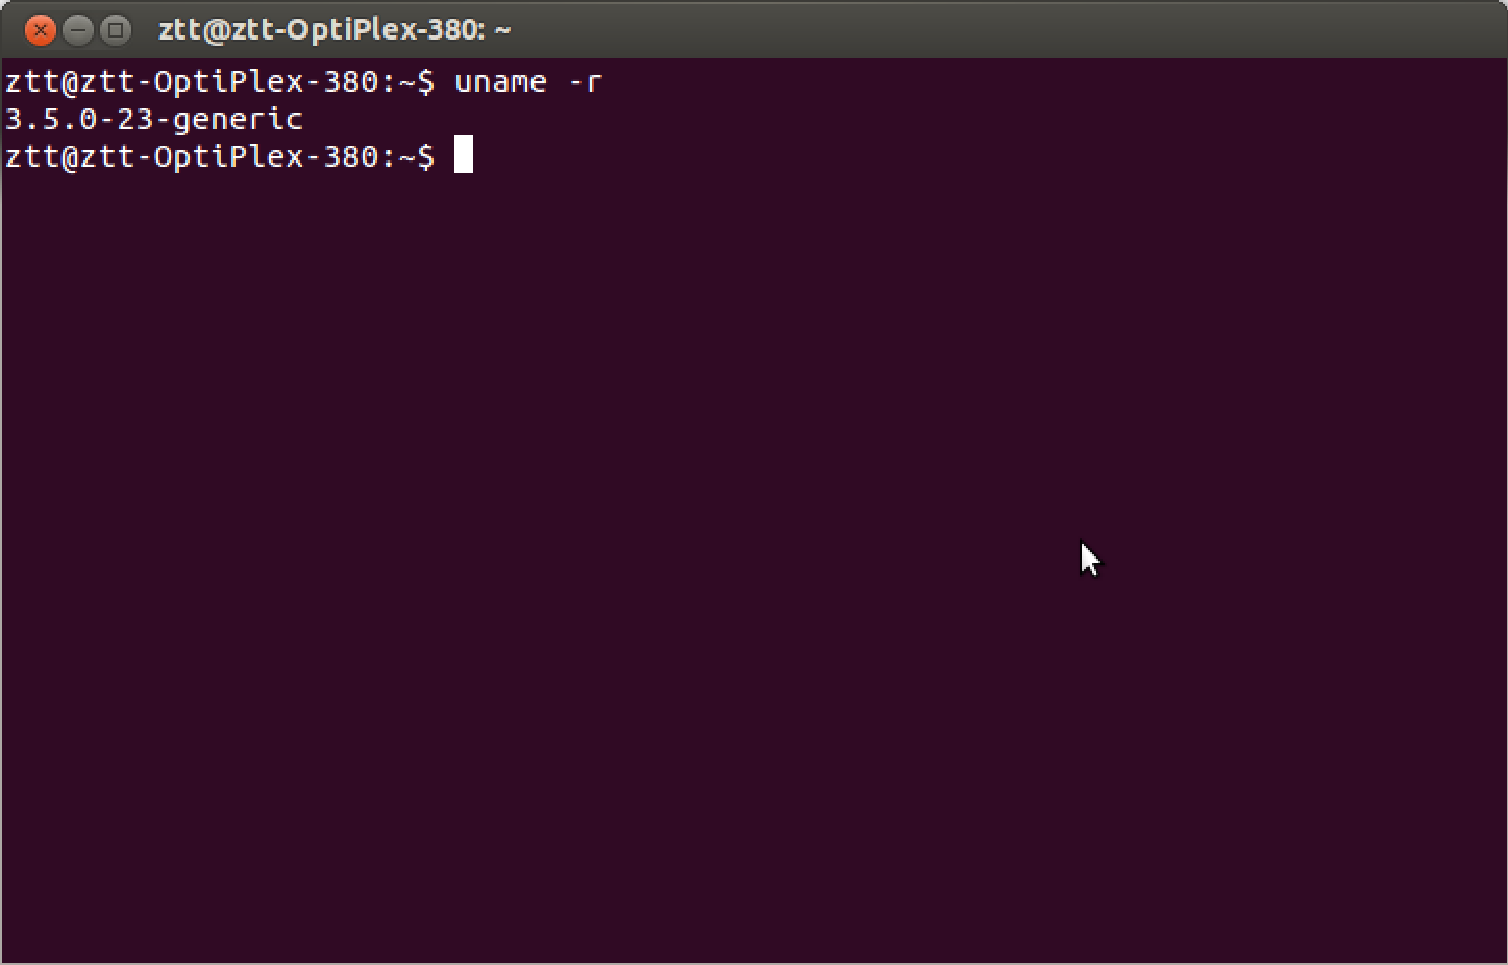
\includegraphics[scale=0.4]{figs/1.pdf}}
    	\subfigure[boot目录下文件]{
    		\label{fig:subfig1:b}
    		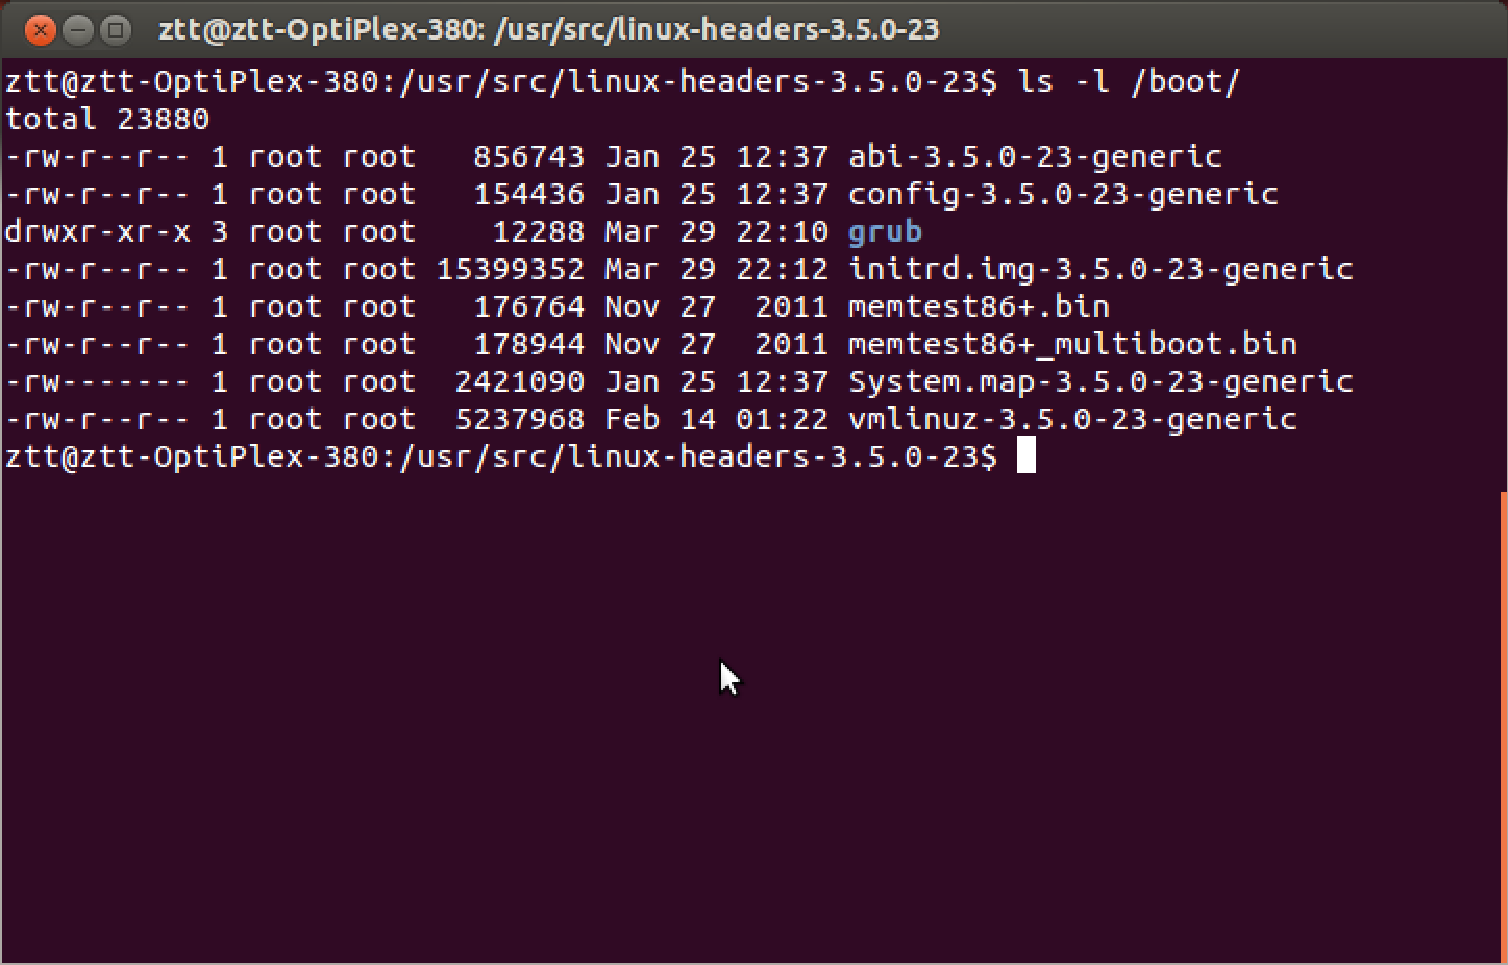
\includegraphics[scale=0.4]{figs/2.pdf}}
    	\label{fig:subfig1}
\end{figure}

\item[下载内核]	\href{http://www.kernel.org}{linux内核官网},建议下载stable的版本--linux-3.8.5.tar.xz

\item[拷贝文件]	将内核文件拷贝到/usr/src目录下.
\begin{lstlisting}[style=BASH]
hjy@jy:~$ sudo cp ~/Downloads/linux-3.8.5.tar.xz /usr/src
\end{lstlisting}

\item[解压文件]	解压.xz格式的文件要用xz\footnote{压缩:xz -z file.tar \& 解压:xz -d file.tar.xz} 命令
\begin{lstlisting}[style=BASH]
hjy@jy:~$ cd /usr/src
hjy@jy:/usr/src$ sudo xz -d linux-3.8.5.tar.xz
hjy@jy:/usr/src$ sudo tar -xvf linux-3.8.5.tar
\end{lstlisting}

\item[清理残留文件]	本步针对已经编译过多次的内核文件.如果是刚刚解开的包,不需要执行这一步
\begin{lstlisting}[style=BASH]
hjy@jy:/usr/src$ cd linux-3.8.5
hjy@jy:/usr/src/linux-3.8.5$ sudo make mrproper
\end{lstlisting}
\end{description}


\subsection{配置内核}
通过图形界面配置\footnote{参考网址:\url{http://forum.ubuntu.org.cn/viewtopic.php?t=134404} \& \url{http://lamp.linux.gov.cn/Linux/kernel_options.html}}
\begin{lstlisting}[style=BASH]
hjy@jy:/usr/src/linux-3.8.5$ sudo make menuconfig
\end{lstlisting}

\underline{\textit{可能出现的错误}:}
\begin{itemize}
\item requires the ncurses libraries.
\begin{lstlisting}[style=BASH]
hjy@jy:/usr/src/linux-3.8.5$ sudo apt-get install libncurses-dev
\end{lstlisting}
\end{itemize}

\begin{itemize}
\item General Setep
\begin{description}
\item[Prompt for development and/or incomplete code/drivers]	如果你的硬件比较新,那几乎是必须选的,这样,我们才可以找到4965无线网卡,alsa声音驱动等等。

\item[Kernel log buffer size]	我选15,双核。如果你用ia64,要选16。

\item[Control Group support]		集群支持?可以不要

\item[Choose SLAB allocator (SLUB (Unqueued Allocator))]	 内存管理模式选择slub
\end{description}


\item Block Layer
\begin{description}
\item[Support for Large Block Devices]	假如没有2TB的硬盘,就去掉

\item[Support for Large Single Files]	也不需要,谁有2TB的文件
\end{description}


\item \underline{Processor type and features}
\begin{description}
\item[Symmetric multi-processing support]	打开多核的开关,cpu是双核的,选中。

\item[Processor family (Core 2/newer Xeon)]	我的是Core 2/newer Xeon。

\item[Generic x86 support]	找到自己的cpu后,把选项去掉。

\item[Subarchitecture Type]	选(PC-compatible)

\item[Maximum number of CPUs]	输入自己的核心数目,我输入2

\item[SMT (Hyperthreading) scheduler support]	超线程技术,P4有支持的,我的t8100不支持,目前大部分市场上的家用cpu都不支持。

\item[High Memory Support (4GB)]	1G以下选1G;我是3G,选4G;4G以上的选16G

\item[Timer frequency]	默认是250Hz,较新的cpu都可以选择了1000Hz,性能更好。
\end{description}


\item Power Management Options
\begin{description}
\item[APM (Advanced Power Management) BIOS support]	现在的电脑都用acpi,去掉

\item[Default CPUFreq governor (conservative)]	cpu节电模式有四个,笔记本默认选conservative比较好。

\item[ACPI Processor P-States driver]	必须选,不然CPU Frequency就不能用。
\end{description}


\item Bus Options
\begin{description}
\item[网卡]	除了我的千兆网卡 Broadcom Tigon3 support和4965无线网卡Intel Wireless WiFi 4965AGN,其余的硬件支持统统去掉。

\item[声卡]	我的是hd声卡,我只是在PCI devices中,选intel hd 声卡,再选Build IDT/Sigmatel HD-audio codec support,除此之外的硬件支持全部去掉。

\item[SCSI device support]	现在都是SATA硬盘,一定要选*

\item[NatSemi SCx200 support]	去掉

\item[Support for PCI Hotplug (EXPERIMENTAL)]	如果没有PCI热插拔设备,去掉.这里的选项可以考虑全部编译进内核,而不是以模块形式存在。
\end{description}


\item \underline{Device Drivers}
\begin{description}
\item[PCI Express support]	现在新买的机器基本上都是PCI Express了

\item[SCSI disk support]		如果你的/boot放在SATA硬盘上,一定要选*。

\item[SCSI CDROM support]	用刻录机,必须选。
\end{description}


\item File Systems
\begin{description}
\item[Filesystem in Userspace support]	是必选的,如果你要用windows分区。

\item[ISO 9660 CDROM file system support]	一般选*

\item[VFAT (Windows-95) fs support]	 有FAT32分区就选*吧

\item[NTFS file system support]	有NTFS分区就选*吧

\item[NTFS write support]	如果想对 NTFS分区进行写操作,选*
\end{description}
\end{itemize}



\subsection{编译内核}
\begin{description}
\item[专用工具]	ubuntu编译内核的工具是make-kpkg,与其他的发行版相比,步骤相对简单.
\begin{lstlisting}[style=BASH]
hjy@jy:/usr/src/linux-3.8.5$ sudo make-kpkg clean
hjy@jy:/usr/src/linux-3.8.5$ sudo make-kpkg -initrd --append-to-version=hjy20130330 kernel_image kernel-headers
\end{lstlisting}

\underline{\textit{可能出现的错误}:}
\begin{itemize}
\item make-kpkg: command not found.
\begin{lstlisting}[style=BASH]
hjy@jy:/usr/src/linux-3.8.5$ sudo apt-get install kernel-package
\end{lstlisting}
\end{itemize}
\end{description}


\subsection{安装内核}
编译完成就是安装工作。编译好的内核在上一层目录。包括linux-headers-...-_i386.deb和linux-image-...-i386.deb两个文件,如果你不搞开发的话,只要安装内核就可以,头文件以后要用的时候再说。
\begin{lstlisting}[style=BASH]
hjy@jy:/usr/src/linux-3.8.5$ cd ..
hjy@jy:/usr/src/$ sudo dpkg -i linux-image-3.8.5+[tab]
\end{lstlisting}


\subsection{重启验证}
\begin{lstlisting}[style=BASH]
hjy@jy:/usr/src/$ sudo reboot
\end{lstlisting}
验证结果\ref{fig:subfig2}
\begin{figure}[!htbp]
	\centering
	\caption{升级内核后}
		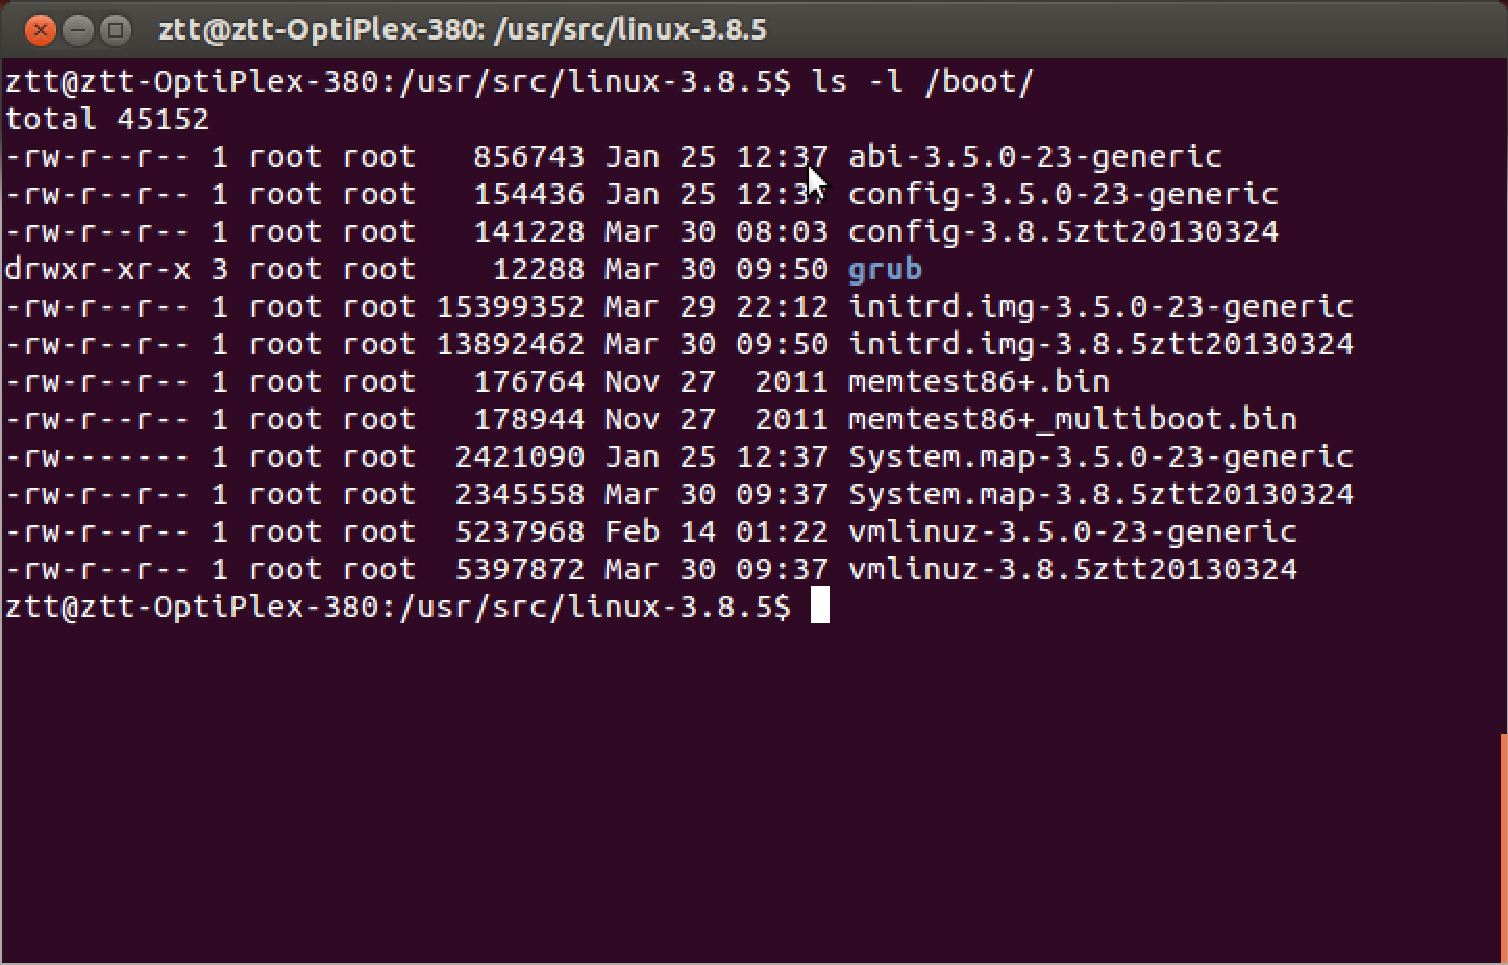
\includegraphics[scale=0.4]{figs/3.pdf}}
    	\label{fig:subfig2}
\end{figure}
\subsection{AFQ}
\subsubsection{准备}
\begin{enumerate}
\item 编译的内核与机器使用的多少位操作系统有关否?\\
答:无关

\end{enumerate}

\clearpage